\documentclass{sig-alternate-ipsn13}

\begin{document}

\title{Passive device-free indoor localisation from RSSI}
%
% You need the command \numberofauthors to handle the 'placement
% and alignment' of the authors beneath the title.
%
% For aesthetic reasons, we recommend 'three authors at a time'
% i.e. three 'name/affiliation blocks' be placed beneath the title.
%
% NOTE: You are NOT restricted in how many 'rows' of
% "name/affiliations" may appear. We just ask that you restrict
% the number of 'columns' to three.
%
% Because of the available 'opening page real-estate'
% we ask you to refrain from putting more than six authors
% (two rows with three columns) beneath the article title.
% More than six makes the first-page appear very cluttered indeed.
%
% Use the \alignauthor commands to handle the names
% and affiliations for an 'aesthetic maximum' of six authors.
% Add names, affiliations, addresses for
% the seventh etc. author(s) as the argument for the
% \additionalauthors command.
% These 'additional authors' will be output/set for you
% without further effort on your part as the last section in
% the body of your article BEFORE References or any Appendices.

% \numberofauthors{2} %  in this sample file, there are a *total*
% of EIGHT authors. SIX appear on the 'first-page' (for formatting
% reasons) and the remaining two appear in the \additionalauthors section.
%
% \author{\vspace{-2cm}
% You can go ahead and credit any number of authors here,
% e.g. one 'row of three' or two rows (consisting of one row of three
% and a second row of one, two or three).
%
% The command \alignauthor (no curly braces needed) should
% precede each author name, affiliation/snail-mail address and
% e-mail address. Additionally, tag each line of
% affiliation/address with \affaddr, and tag the
% e-mail address with \email.
%Markus~Matoni,
%         Michael~Krawez,
%         Gipsa~Joseph
%         and~Stephan~Sigg
% 1st. author
% \alignauthor
% 
% Markus Matoni, Michael Krawez, Gipsa Joseph\\
%        \affaddr{University of Goettingen}\\
% % 2nd. author
% % \and  % use '\and' if you need 'another row' of author names
% % 4th. author
% \alignauthor Stephan Sigg\\
%        \affaddr{University of Goettingen}\\
%        \affaddr{Networking Group}\\
%        \email{ssigg@gwdg.de}
% }
% There's nothing stopping you putting the seventh, eighth, etc.
% author on the opening page (as the 'third row') but we ask,
% for aesthetic reasons that you place these 'additional authors'
% in the \additional authors block, viz.
% Just remember to make sure that the TOTAL number of authors
% is the number that will appear on the first page PLUS the
% number that will appear in the \additionalauthors section.

\maketitle
\begin{abstract}
We propose a device-free passive indoor localisation system by analysing the fluctuation in received RSSI packets received from environmental WiFi access points.
With a single device in each room the system is able to detect presence and to provide a broad classification of the actual location of a single person dividing the room into a grid of four regions. 
\end{abstract}


  \section{Extended abstract}
  Device-Free Localisation (DFL) was defined by Youssef et al. as the localisation or tracking of a person using RF-Signals while the entity monitored is not required to carry an active transmitter or receiver~\cite{Pervasive_Youssef_2007}.
  They initially considered fluctuation in the direct link between WiFi devices in order to track movement that physically intercepts this line-of-sight connection.
  By separating the sensed region into a grid of clusters, Wilson et al.~\cite{RFSensing_Wilson_2009} achieved an average error of about $0.5$~meters.
  Later, Zhang et al. could demonstrate a high accuracy of below 1m for the simultaneous tracking of five moving targets by isolating the LoS path between nodes~\cite{Pervasive_Zhang_2012}.

%   But RSSI has also been utilised for the recognition of other purposes such as the monitoring of breathing frequency~\cite{Pervasive_Patwari_2011b}, the recognition of activities~\cite{Pervasive_Scholz_2013} or attention~\cite{Pervasive_Shi_2014}.

%   Common to all these studies is that they utilize active systems incorporating transmit and receive devices.
  Recently, the recognition of capabilities of a passive, single receiver RSSI-based recognition system have been reported~\cite{Pervasive_Sigg_2014}
  They demonstrated the potential of such a system to recognise presence and distance of movement to a receive device.
  In this demo, we utilise a similar approach for indoor localisation.

  \section{System description}
  Our system utilises fluctuation in received RSSI packets from environmental WiFi access points for the detection of movement in the proximity of receive devices. 
  It consists of receive devices placed in each room and a mobile monitoring point that displays the sensed activities. 
  As receive devices we utilise Nexus One mobile phones.
  These phones constantly monitor RSSI packets from environmental WiFi access points via tcpdump.\footnote{The access points are not part of our installation.}
  On the phones, the captured stream of packets is pre-processed to filter the RSSI of only meaningful packets.
  This data is regularly broadcast to the mobile device utilised as monitoring point.
  At the monitoring point, the various data streams are then further processed to distinguish the presence of individuals in specific rooms as well as heir relative location towards the receive device. 
  We attempt to distinguish up to four distinct areas in a single room.
%   This scenario is depicted in figure~\ref{figureScenario}.
%   \begin{figure}
%   \includegraphics[width=\columnwidth, height=6cm]{Figures/sketch.png}
%   \caption{Schematic illustration of a possible instrumentation of the system}
%   \label{figureScenario}
%   \end{figure}
  Main parts of the processing are implemented in python. 
  For the machine learning part we utilise classifiers from the Orange data mining tool.



%
% The following two commands are all you need in the
% initial runs of your .tex file to
% produce the bibliography for the citations in your paper.
\bibliographystyle{abbrv}
\bibliography{/home/stephan/Daten/Arbeit/Veroeffentlichungen/Literatur/Literatur_080128_v2_STS.bib}  % sigproc.bib is the name of the Bibliography in this case
% You must have a proper ".bib" file
%  and remember to run:
% latex bibtex latex latex
% to resolve all references
%
% ACM needs 'a single self-contained file'!
%
%APPENDICES are optional
%\balancecolumns
% \appendix
%Appendix A

% Appendix goes here.

% That's all folks!
\end{document}
